\section{Strain}

When forces are applied to a body, \textbf{deformation}, the change in length or shape, occurs. The change in length, divided by the original length, is the \textbf{strain}. We use strain to \textbf{normalize deformations} with respect to the size of the geometry.

\subsection{Units}

Dimensionless [mm/mm, in/in, or \%]

\subsection{Normal Strain}

\begin{figure*}[!h]
\centering
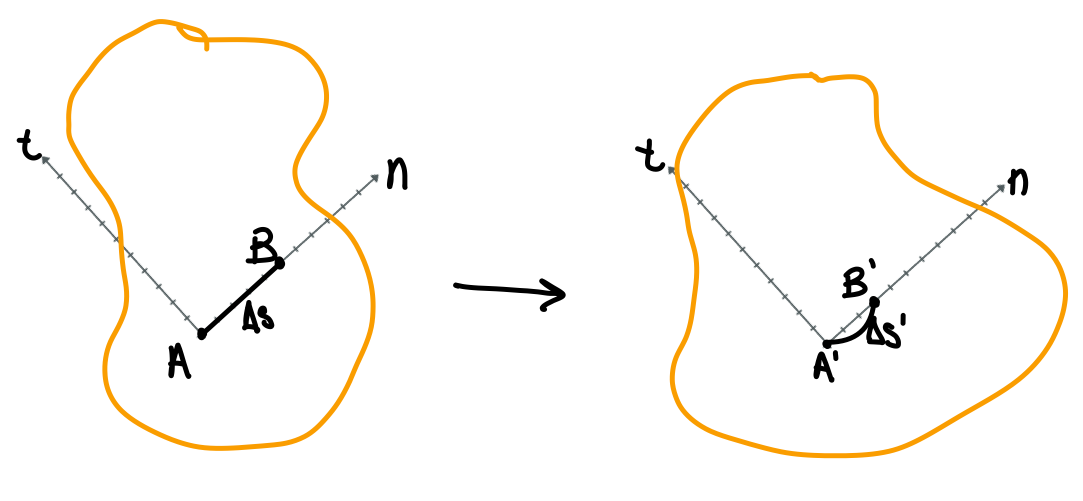
\includegraphics[angle=0, width=3.5in]{Strain-Figures/Normal Strain.png}
\vspace{-2mm}
\caption{\small Normal strain}
\vspace{-3mm}
\label{Fig:Normal Strain}
\end{figure*}

Relative change in \textbf{length} of a line element oriented in arbitrary direction $n$.

\[ \varepsilon_n = lim_{B  \xrightarrow{} A \rm\ along \rm\ n} \frac{\Delta s - \Delta s'}{\Delta s} \]

% \[ \varepsilon_n = lim_{B-&gt;A \rm\ along \rm\ n} \frac{\Delta s = \Delta s&#39;}{\Delta s} \]

\subsubsection{Average Normal (extensional) Strain}

\begin{figure*}[!h]
\centering
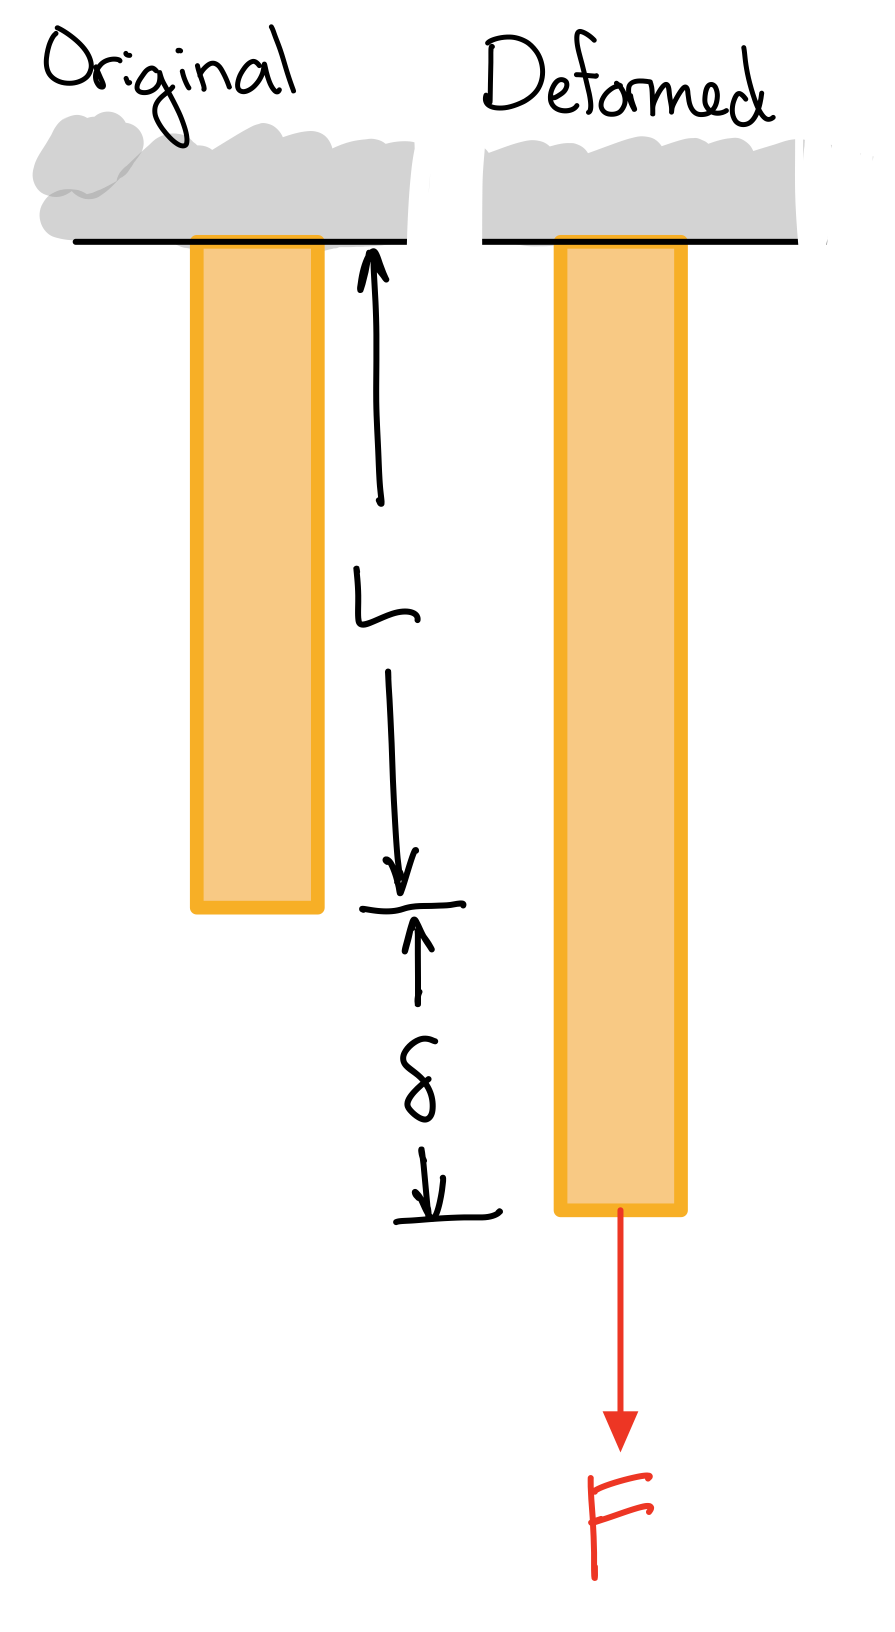
\includegraphics[angle=0, width=2in]{Strain-Figures/Avg Normal Strain.png}
\vspace{-2mm}
\caption{\small Average normal strain}
\vspace{-3mm}
\label{Fig:Avg Normal Strain}
\end{figure*}

\noindent Length change divided by total length.

\[ \epsilon_n = \frac{\delta}{L}\]

\begin{itemize}
    \item \textbf{Engineering} or nominal (normal) strain: Average normal strain using the original (undeformed) total length.
    \[ \varepsilon_{eng} = \frac{\delta}{L_0}\] 
    \item \textbf{True} (normal) strain: Integrate infinitesimal normal strains.
    \begin{figure*}[!h]
    \centering
    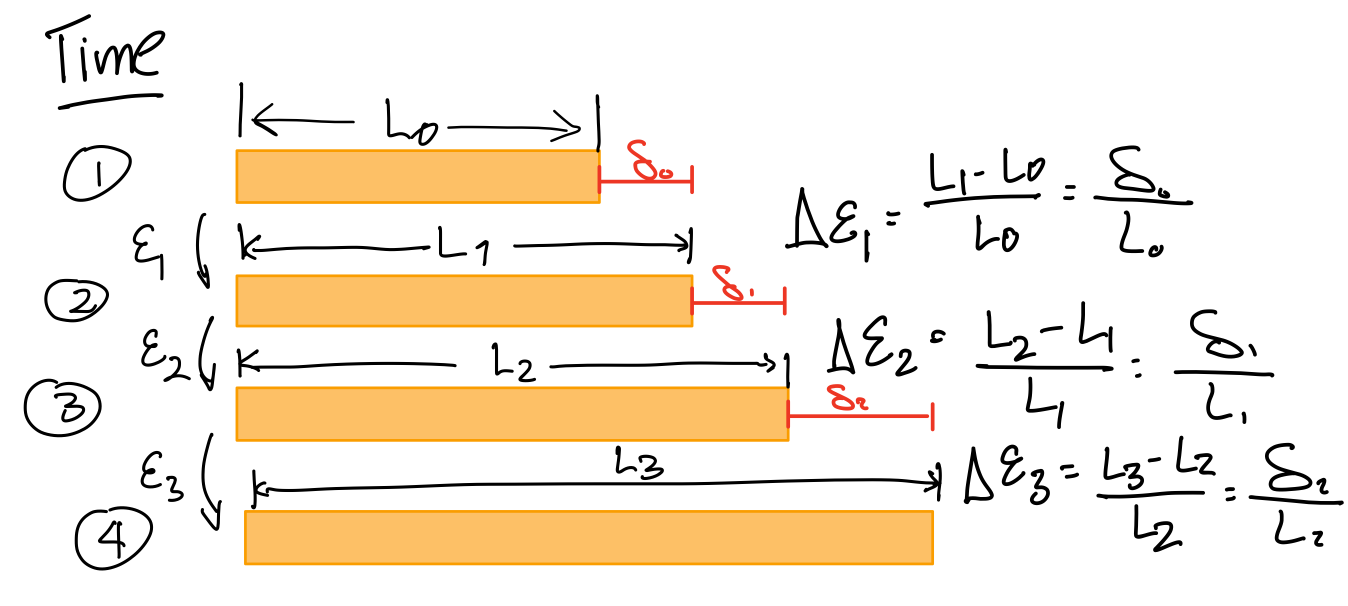
\includegraphics[angle=0, width=4in]{Strain-Figures/True Strain.png}
    \vspace{-2mm}
    \caption{\small True strain}
    \vspace{-3mm}
    \label{Fig:True Strain}
    \end{figure*}

    \[ \varepsilon_{true} = ln(1 + \frac{\delta}{L_0})\]

     \textbf{*Expandable derivation*}
    \[ \varepsilon_{true} = \Sigma\Delta\varepsilon_0 = \int d\varepsilon\]
    \[ \varepsilon_{true} = \int_{L_0}^{L_f}\frac{1}{L}dL\]
    \[ \varepsilon_{true} = ln(L)|_{L_0}^{L_f} = ln(\frac{L_f}{L_0}) \]
    \[ \varepsilon_{true} = ln(\frac{L_0+\delta}{L_0}) = ln(1+\frac{\delta}{L_0})\]
    \[ \varepsilon_{true} = \varepsilon_{eng}-\frac{1}{2}\varepsilon_{eng}^2 + \frac{1}{3}\varepsilon_{eng}^{3} + ...\]
    \textbf{**End Derivation**}
    \item For small strain: $\varepsilon_{true} \approx \varepsilon_{eng}$
\end{itemize}

\subsection{Shear Strain}
Change in \textbf{angle} between line segments oriented in perpendicular directions $n$ and $t$:

\begin{figure*}[!h]
\centering
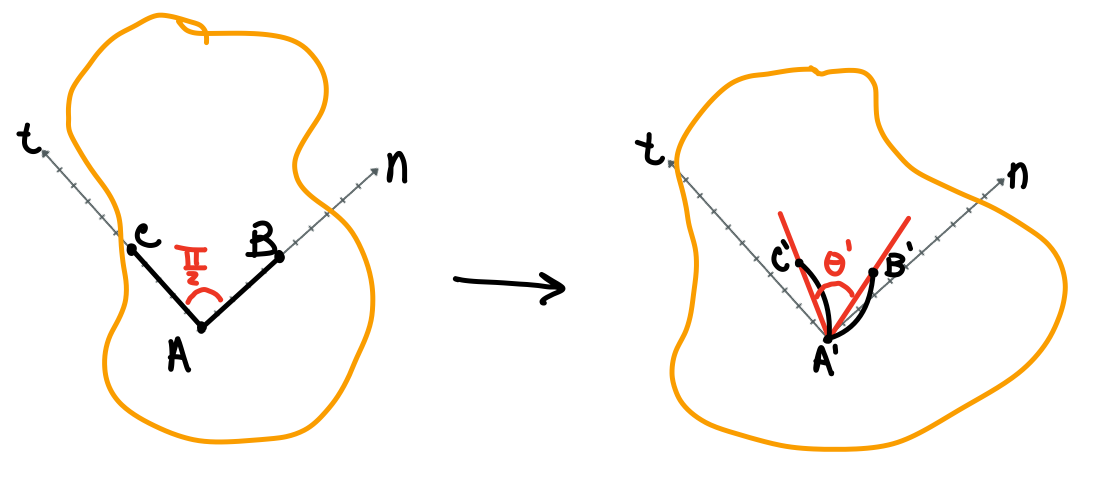
\includegraphics[angle=0, width=3.5in]{Strain-Figures/Shear Strain.png}
\vspace{-2mm}
\caption{\small Shear strain}
\vspace{-3mm}
\label{Fig:Shear Strain}
\end{figure*}

\[ \gamma_{nt} = lim_{\begin{matrix} B \xrightarrow{} A \rm\ along \rm\ n\\ C \xrightarrow{} A \rm\ along \rm\ t \end{matrix}} (\frac{\pi}{2} - \theta') \]

% \[ \gamma_{nt} = lim_{\begin{matrix} B-&gt;A \rm\ along \rm\ n\\ C-&gt;A \rm\&nbsp;along \rm\ t \end{matrix}} (\frac{\pi}{2} - \theta &#39;) \]

\noindent When strains are small, the small angle approximation, $\sin(\theta)\approx \theta$, results in

\[\gamma = \frac{\pi}{2} - \theta \approx \frac{\delta}{L}\]

\subsubsection{Average Shear Strain}

\begin{figure*}[!h]
\centering
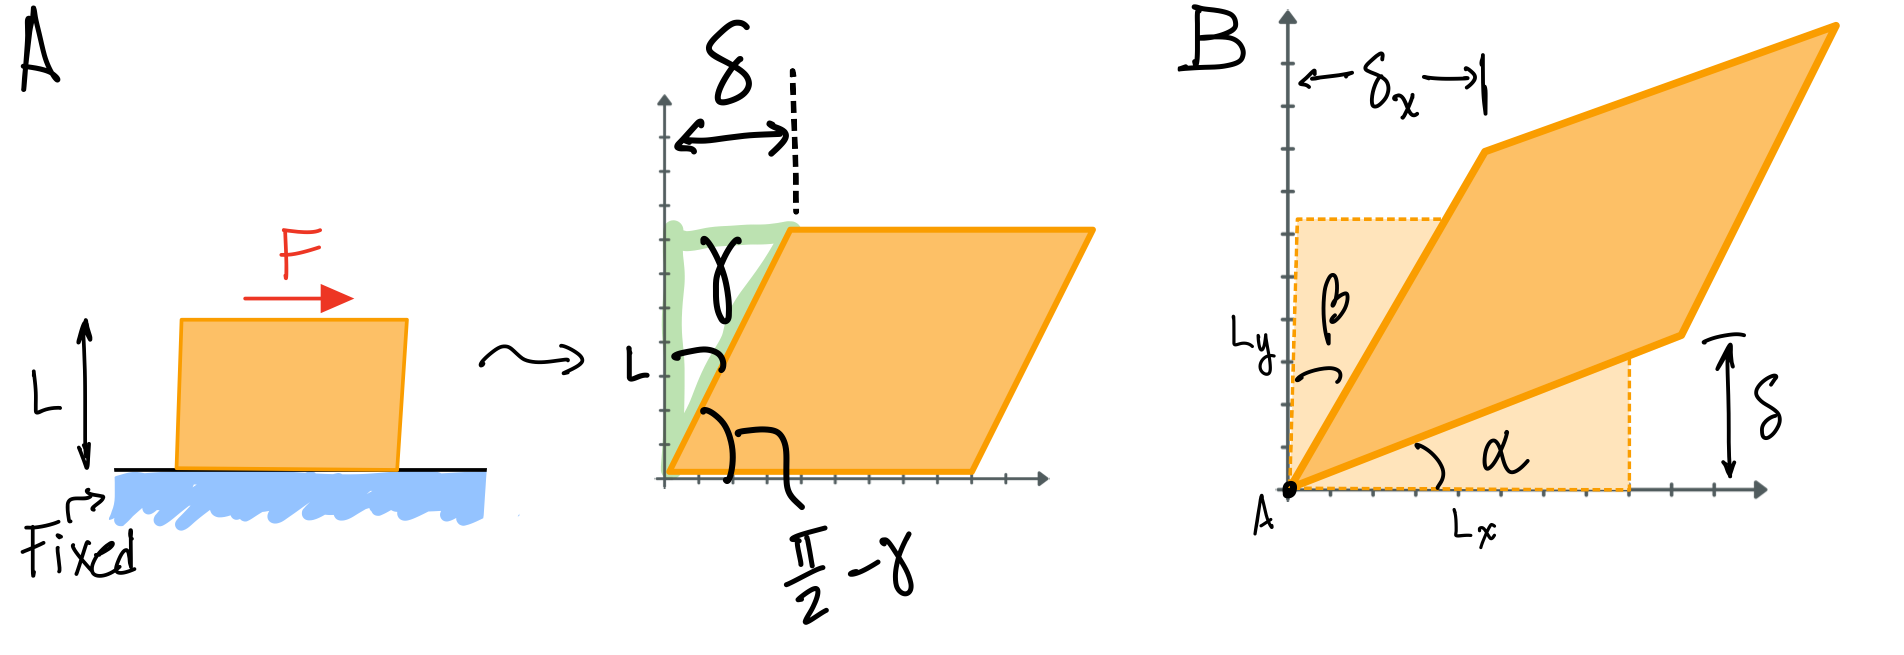
\includegraphics[angle=0, width=5in]{Strain-Figures/Avg Shear Strain.png}
\vspace{-2mm}
\caption{\small Average shear strain}
\vspace{-3mm}
\label{Fig:Avg Shear Strain}
\end{figure*}

\noindent  Fig: \ref{Fig:Avg Shear Strain}A
\[tan(\gamma) = \frac{\delta}{L} \xrightarrow{} \gamma = \frac{\delta}{L}\]
\noindent Fig: \ref{Fig:Avg Shear Strain}B
\[\gamma = \alpha + \beta\]
\[\gamma = \frac{\delta_x}{L_y} + \frac{\delta_y}{L_x}\]


\begin{itemize}
    \item \textbf{Engineering} (shear) strain: Compute angle from length changes and original (undeformed) total length.
    \item \textbf{True} (shear) strain: Integrate infinitesimal angle changes.
\end{itemize}


\subsection{Strain Tensor}
The components of normal and shear strain can be combined into the strain tensor. This is a symmetric matrix.

\[ E = \begin{bmatrix} \varepsilon_{x} & \gamma_{xy} & \gamma_{xz} \\ \gamma_{yx} & \varepsilon_{y} &\gamma_{yz} \\ \gamma_{zx} & \gamma_{zy} &\varepsilon_{z} \end{bmatrix} \]

%\[ E&nbsp;= \begin{bmatrix} \varepsilon_{x} &amp; \gamma_{xy} &amp; \gamma_{xz} \\ \gamma_{yx} &amp; \varepsilon_{y} &amp; \gamma_{yz} \\ \gamma_{zx} &amp;\gamma_{zy} &amp; \varepsilon_{z} \end{bmatrix} \]


\begin{itemize}
    \item  Three normal strain components: $\varepsilon_x, \varepsilon_y, \varepsilon_z$
    \item Six shear strain components: $\gamma_{xy} =\gamma_{yx}, \gamma_{xz}=\gamma_{zx}, \gamma_{yz}=\gamma_{zy}$
\end{itemize}


\noindent The first subscript describes the surface \textbf{orientation} in the normal direction. The second subscript describes the \textbf{direction} of the stress.

\subsection{Measurement of Strain}

\subsubsection{Direct Measurement}

Initial and final lengths of some section of the specimen are measured, perhaps by some handheld device such as a ruler. Axial strain computed directly by following formula:

\[\varepsilon = \frac{\delta}{L} = \frac{L_{final} - L_{initial}}{L_{initial}} \]

\noindent Accurate measurements of strain in this way may require a fairly large initial length.

\subsubsection{Contact Extensometer}

A clip-on device that can measure very small deformations. Two clips attach to a specimen before testing. The clips are attached to a transducer body. The transducer outputs a voltage. Changes in voltage output are converted to strain.

\clearpage

\begin{figure*}[!h]
\centering
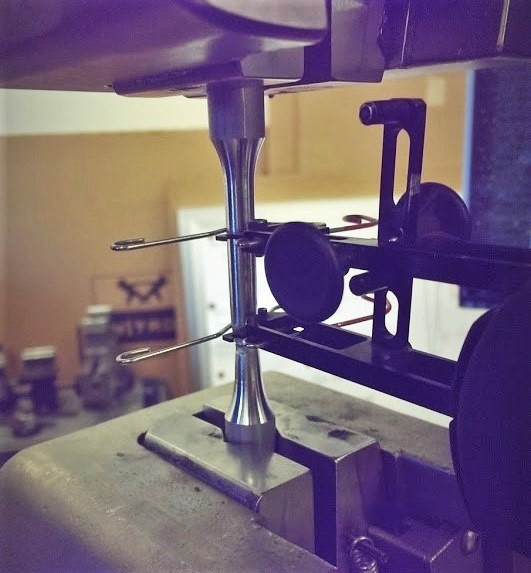
\includegraphics[angle=0, width=2in]{Strain-Figures/extensometer.jpg}
\vspace{-2mm}
\caption{\small A tensile test in the Materials Testing Instructional Laboratory, Talbot Lab, UIUC}
\vspace{-3mm}
\label{Fig:extensometer}
\end{figure*}

\subsubsection{Classic Strain Gauges}

Small electrical resistors whose resistance charges with strain. Change in resistance can be converted to strain measurement. Often sold as "rosettes", which can measure normal strain in two or more directions. Can be bonded to test specimen.

\begin{figure*}[!h]
\centering
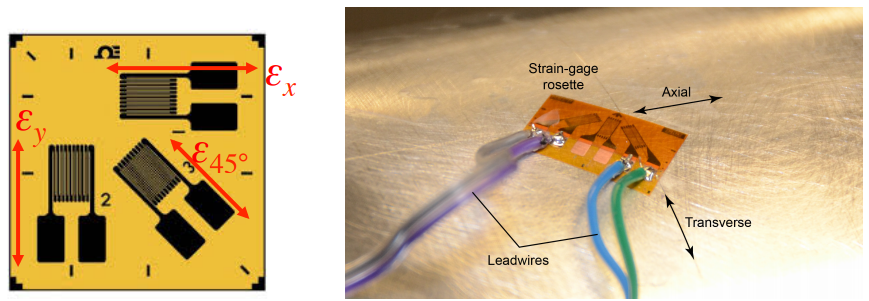
\includegraphics[angle=0, width=4in]{Strain-Figures/strainGauge.png}
\vspace{-2mm}
\caption{\small Rosette strain gauge arrangement and example}
\vspace{-3mm}
\label{Fig:StrainGauge}
\end{figure*}

\subsubsection{Vibrating Wire Strain Gauge}
A calibrated wire is set into vibration and its frequency is measured. Small changes in the length of the wire as a result of strain produce a measurable change in frequency, allowing for accurate strain measurements over relatively long gauge lengths.

\begin{figure*}[!h]
\centering
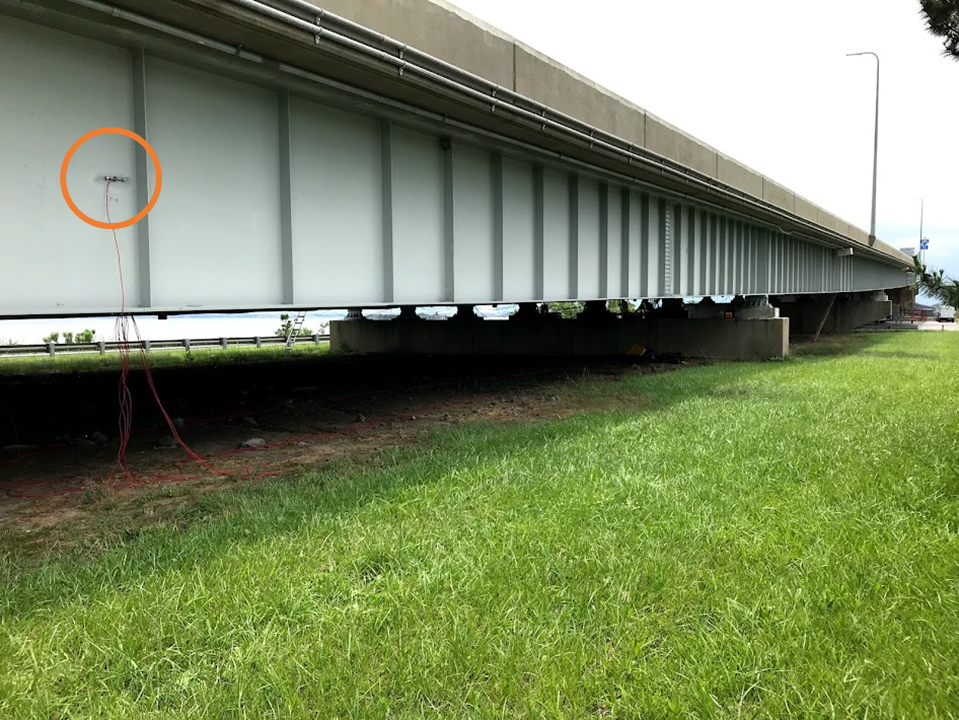
\includegraphics[angle=0, width=3in]{Strain-Figures/VibratingWire.png}
\vspace{-2mm}
\caption{\small Vibrating wire strain gauge attached to the side of a bridge}
\vspace{-3mm}
\label{Fig:VibeWire}
\end{figure*}

\subsubsection{Digital Image Correlation (DIC)}

Image placed on surface of test specimen. Image may consist of speckles or some regular pattern. Deformation of image tracked by digital camera. Image analysis used to determine multiple strain component.

\begin{figure*}[!h]
\centering
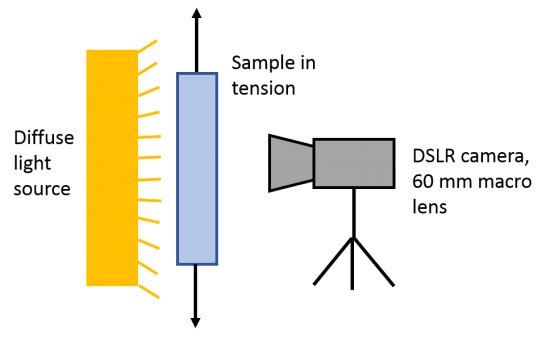
\includegraphics[angle=0, width=3in]{Strain-Figures/dic.png}
\vspace{-2mm}
\caption{\small Experiment set up. The diffuse light source consists of two fluorescent tube lights that produce white light, behind a translucent plastic sheet.}
\vspace{-3mm}
\label{Fig:dic}
\end{figure*}

\begin{figure*}[!h]
\centering
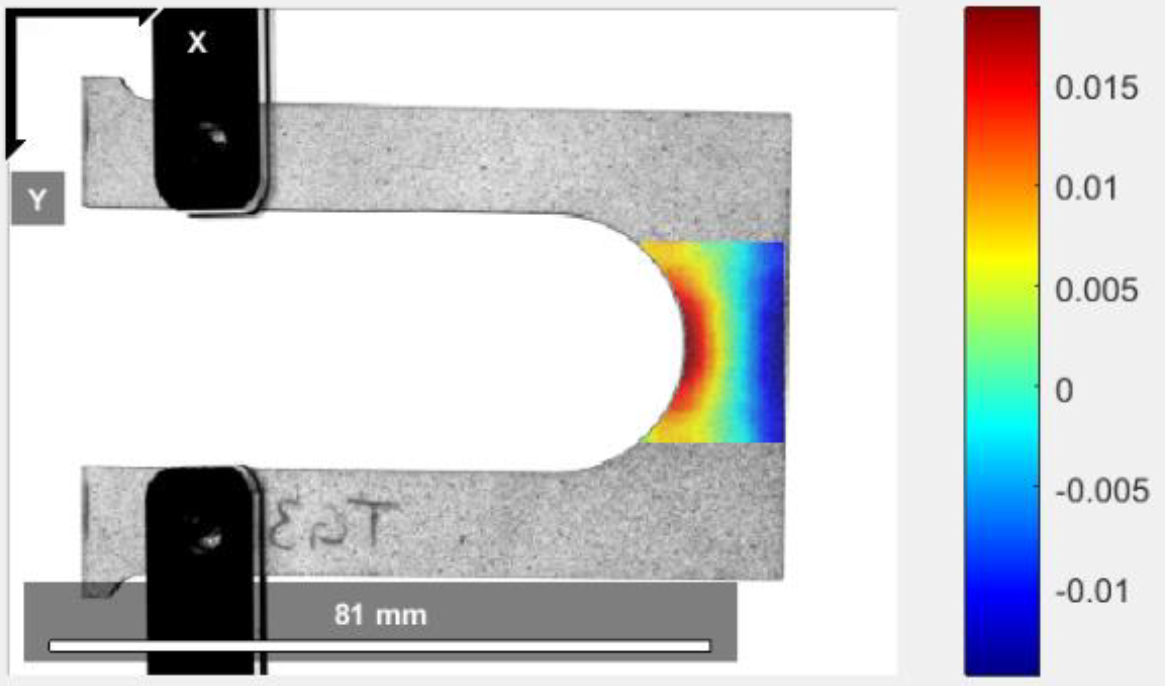
\includegraphics[angle=0, width=4in]{Strain-Figures/dic2.png}
\vspace{-2mm}
\caption{\small $\varepsilon_{yy}$ strain calculated through DIC of straight-curved specimen with an applied load of 114 N from TAM 456, UIUC.}
\vspace{-3mm}
\label{Fig:dic2}
\end{figure*}

